% author: Simon Bachmann

\section{Social Trust Certificates}\label{section:social-trust-certificates}

A decentralized ticketing platform does not restrict any user from creating an event on the distributed ledger. Thus, a mechanism must be developed to mitigate fraudulent events.

A common design pattern for this problem is an on-chain voting mechanism. Usually these decentralized platforms create a multi purpose token for this. One of the tokens functions is governance. Token holders are eligible to cast votes if they think an event is fraudulent and in return they receive maintenance fees. However, this requires that the event creator must deposit some currency when creating an event. Furthermore, people must make an on-chain transaction to vote on suspicious events. This makes the UX more complex for the event host. Introducing a new token for every decentralized  app also results in a fragmented ecosystem.

The goal is to enable users to check whether an event is legit or not without the need of a governance mechanism. Furthermore, the level of trust that is needed from third parties must not be greater than in the current ticketing ecosystem. 

Social trust certificates enable a user to check whether the event is legitimate or not without the need of a third party. Event hosts upload the same public key, that is used for creating the event, to a social profile or the official event website. This way, an event host can proof his ownership of the event as well as the social profile or website. 

Event guests can retrieve the url of the website or social profile from the smart contract and then verify themselves, if the event is legitimate or not. However, this is not 100\% foolproof. For an imposter it is easy to fake an official website with a slightly different url and buy followers on social media platforms. However, this threat already exists today. Aggregating multiple social media platforms makes it harder for an attacker and thus, increases the legitimacy of an event compared to today's standards. 

Figure \ref{fig:trust-certificate-event-website} illustrates how the event host can use the official event website to increase the authenticity of the event. 

\begin{figure}[H]
    \centering
    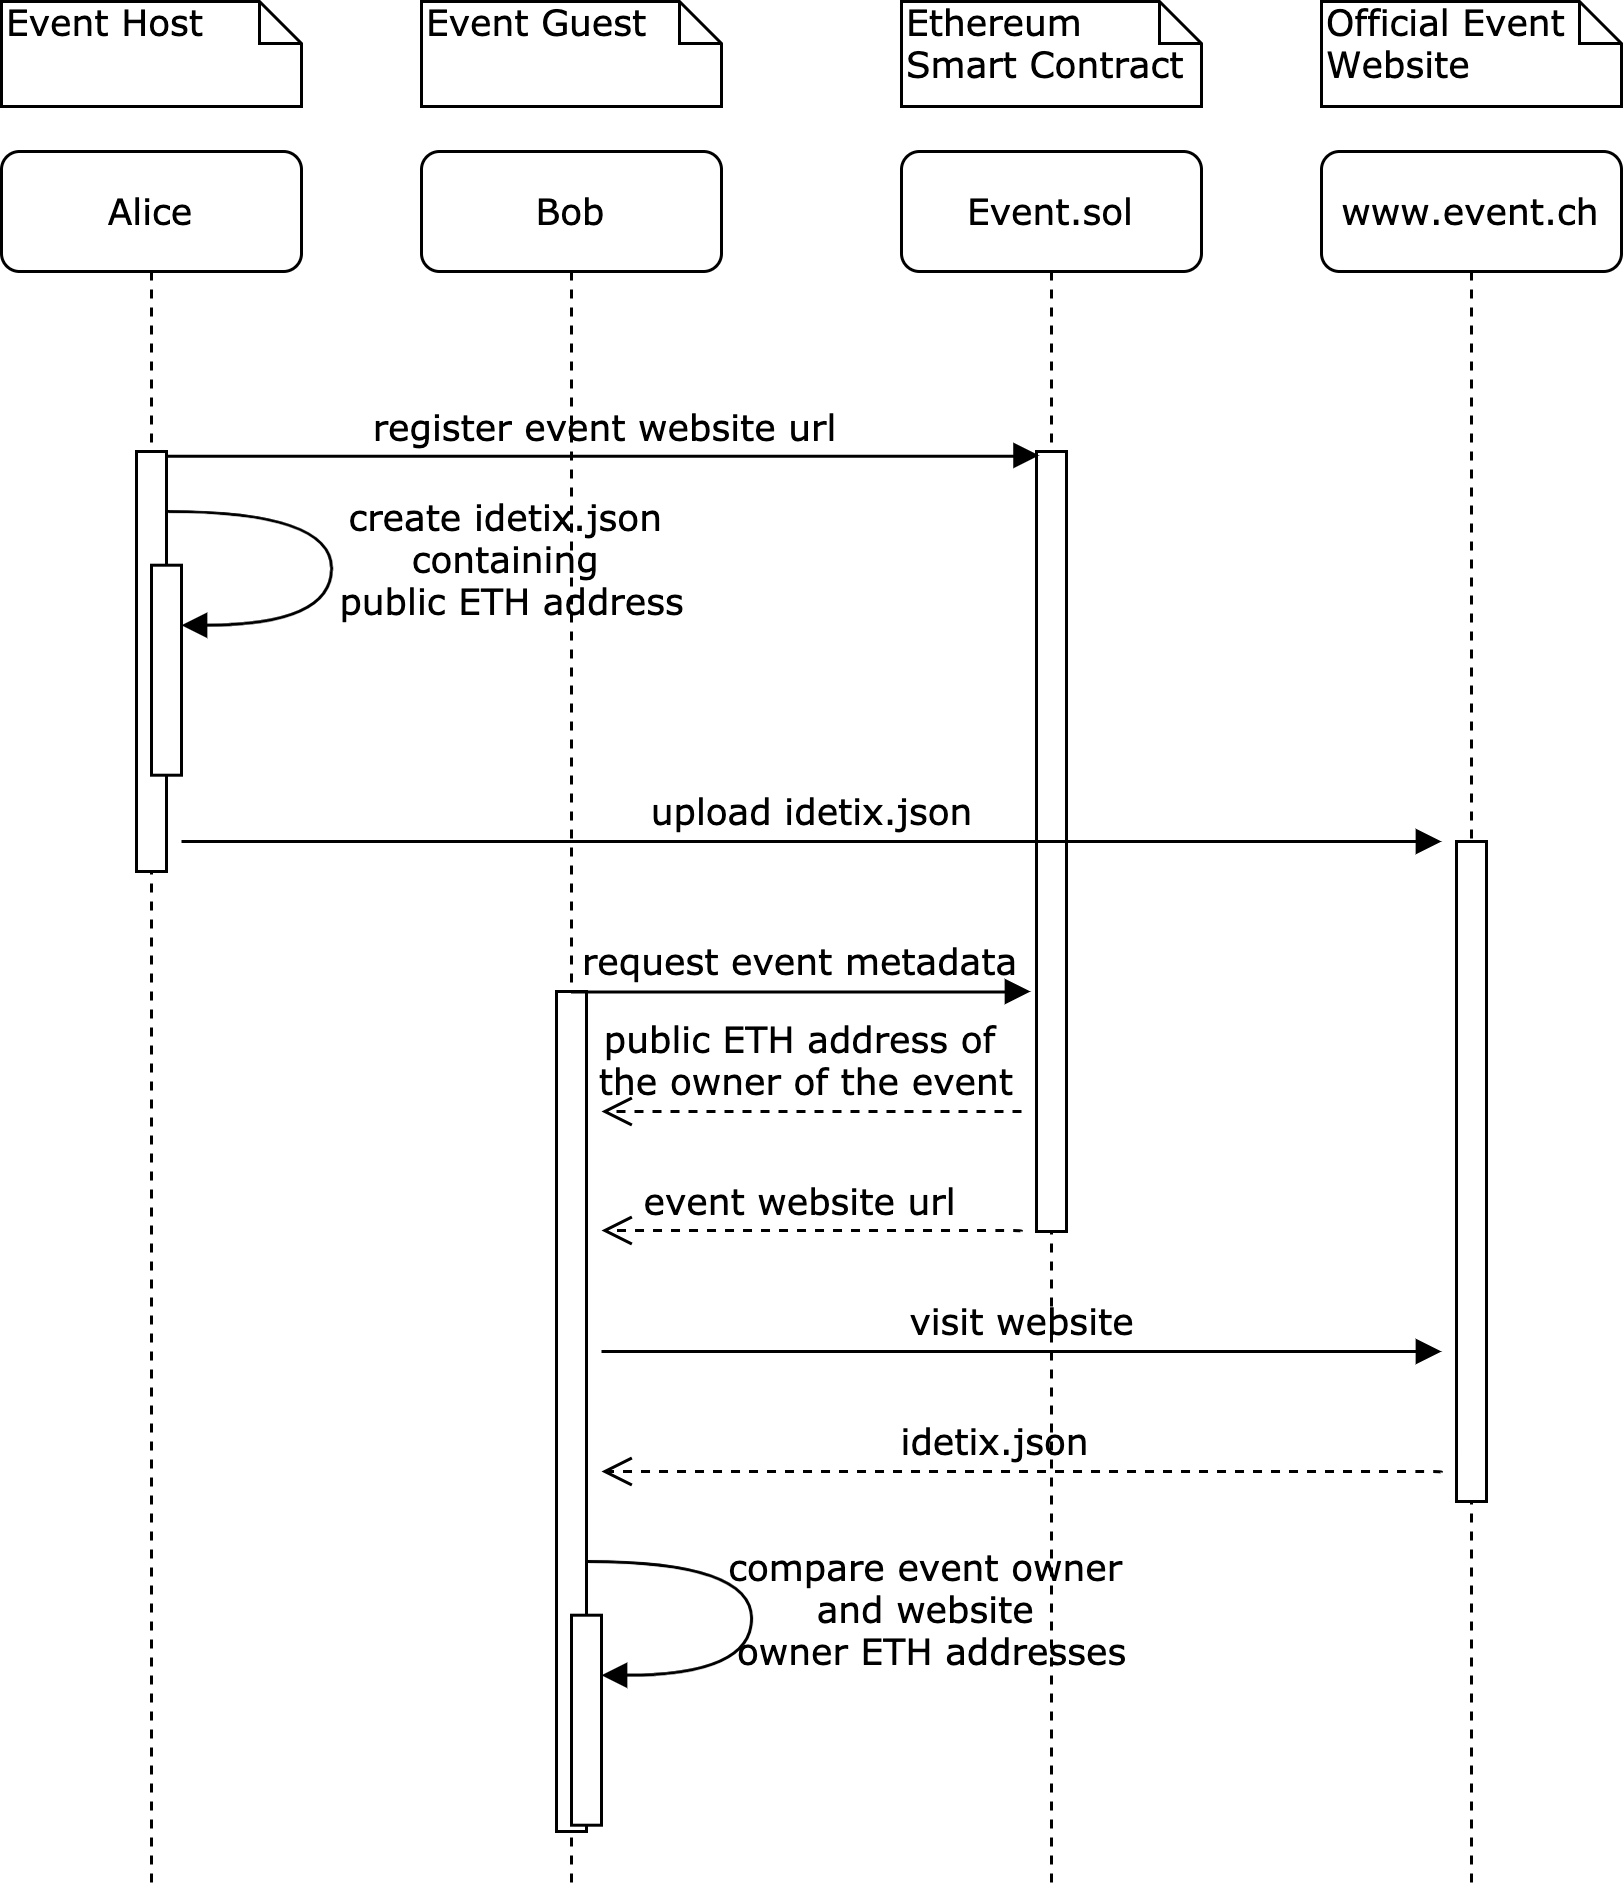
\includegraphics[width=14cm]{figures/social-trust-certificates.png}
    \caption{Social Trust Certificated on the Event Website}
    \label{fig:trust-certificate-event-website}
\end{figure}

Similarly, this procedure can be applied to any social profile such as Twitter, Facebook, Instagram and other social media platforms. Instead of uploading a JSON file or html meta-tag to the website, the public address is included in the profile description on that particular social media platform. 